\chapter{Sistema Linear}

Denomina-se \textbf{sistema linear $m \times n$} o conjunto $S$ de $m$ equações lineares (equações de 1º grau) em $n$ incógnitas (variáveis), que pode ser representado assim:
\[S= \begin{cases}
      a_{11}x_1 + a_{12}x_2 + \cdots + a_{1n}x_n = b_1 \\
      a_{21}x_1 + a_{22}x_2 + \cdots + a_{2n}x_n = b_2 \\
      \vdots \\
      a_{m1}x_1 + a_{m2}x_2 + \cdots + a_{mn}x_n = b_m \\
     \end{cases} \]

Dizemos que $(\alpha_1, \alpha_2, \cdots, \alpha_n)$ é \textbf{solução} de um sistema linear quando $(\alpha_1, \alpha_2, \cdots, \alpha_n)$ é solução de cada uma das $m$ equações do sistema.

\section{Sistema de duas equações lineares}

\vskip0.3cm
 \colorbox{azul}{
 \begin{minipage}{0.9\linewidth}

  Em particular uma equação em duas variáveis $x$ e $y$ é da forma $ax + by= c$ onde $a, b$ e $c$ são constantes reais e $a$ e $b$ não são simultaneamente nulos. Assim ao consideramos duas destas equações
  \[S= \begin{cases}
      a_1x + b_1y= c_1 \\
      a_2x + b_2y= c_2
     \end{cases}\]
 temos um sistema linear de duas equações lineares e duas incógnitas. Um par de valores $x$ e $y$, frequentemente representado pelo par ordenado $(x, y)$, que satisfaz as duas equações, quando existe, é chamado de solução do sistema.

 \end{minipage}}
 \vskip0.3cm

\begin{exem}
 Considere o sistema $S_1$ dado por:
 \[S_1= \begin{cases}
      -x + 2y= 1 \\
      x + y= 8,
     \end{cases}\]
 note que o par ordenado $(5, 3)$ é solução deste sistema já que:
 \[S_1= \begin{cases}
      -5 + 2 \cdot 3= 1 \\
      5 + 3= 8
     \end{cases} .\]

Já o par ordenado $(3, 5)$ não é solução do sistema $S_1$ pois:
\[S_1= \begin{cases}
      -3 + 2 \cdot 5= 7 \neq 1 \\
      3 + 5= 8
     \end{cases} .\]
\end{exem}

Existem várias formas de resolver um sistema linear, vamos aqui apresentar duas delas, e depois discutiremos como interpretamos geometricamente as soluções de um sistema linear de duas equações e duas incógnitas.

\begin{enumerate}[A)]
 \item \textbf{Método da adição ou subtração}

 Em resumo a ideia deste método é multiplicar cada uma das duas equações do sistema por uma constante, de forma que as equações resultantes tenham os coeficientes de uma das incógnitas numericamente iguais. Caso os sinais dos coeficientes sejam distintos, some as equações; se forem o mesmo, subtraia-as, com isso ficamos com uma equação de 1º grau com apenas uma incógnita, a qual sabemos resolver, com sua solução em mãos podemos substituir em qualquer uma das duas equações iniciais e resolvê-la obtendo assim o valor da outra incógnita, e consequentemente temos a solução do sistema, assim como fazemos no seguinte exemplo que ilustra exatamente este método de resolução de sistema.

 \[S= \begin{cases}
      2x - y= 4 \ \ (\cdot 2)\\
      x + 2y= -3
     \end{cases}\]

$$\begin{tabular}{cccccc}
   & 4x & -  & 2y  & =  & 8  \\
 + & x & + & 2y & = & -3 \\\hline
   & 5x & + & 0 & = & 5 \\
\end{tabular}$$

\[5x= 5 \Rightarrow x=1.\]
Substituindo $x=1$ na segunda equação obtemos:
\[x + 2y= -3 \Rightarrow 1 + 2y= -3 \Rightarrow 2y = -3 -1 \Rightarrow 2y= -4 \Rightarrow y=-2.\]
Assim o par ordenado $(x, y)= (1, -2)$ é solução do sistema.

 \item \textbf{Método da substituição}

 Neste método a ideia é ``isolar" uma das incógnitas em uma das equações e substituir na outra, chegando assim em uma equação de 1º grau com uma variável, a qual sabemos resolver, ao resolver esta última equação retornamos a solução encontrada na equação anterior para encontrar o valor da outra variável. Detalhamos este método no seguinte exemplo.

 \[S= \begin{cases}
      2x - y= 4 \ \ (I)\\
      x + 2y= -3 \ \ (II)
     \end{cases}\]

 Isolando $y$ em $(I)$ obtemos:
 \[2x - y= 4 \Rightarrow -y = 4 -2x \Rightarrow y = 2x -4\]
 substituindo em $(II)$ temos:
 \[x + 2y= -3 \Rightarrow x + 2(2x - 4)= -3 \Rightarrow x + 4x - 8= -3 \Rightarrow 5x= -3 + 8 \Rightarrow 5x=5 \Rightarrow x=1\]
 voltando $x= 1$ em $(I)$ temos $y= 2 \cdot 1 - 4 \Rightarrow  y= 2 -4 \Rightarrow y= -2$.

 Assim o par ordenado $(x, y)= (1, -2)$ é solução do sistema.
\end{enumerate}

\textbf{Interpretação geométrica dos sistemas lineares $2 \times 2$}

Note que, dada uma equação $ax + by= c$, de 1º grau em duas variáveis, podemos isolar $y$ obtendo assim que
\[y= \frac{c - ax}{b}= \frac{c}{b} - \frac{ax}{b},\]
que fazendo $y= f(x)$ pode ser interpretada como uma função do 1º grau, cujo gráfico é uma reta, logo o gráfico de $ax + by= c$ é uma reta. Entendendo isso temos que ao resolver um sistema de duas equações e duas incógnitas, quando o mesmo tem solução, estamos procurando as coordenadas do ponto de interseção das duas retas, cujas equações são dadas pelas equações do sistema.

Porém dadas duas retas quaisquer no plano existem três possíveis posições relativas entre estas duas retas, que são: coincidentes, paralelas e concorrentes. Assim considerando o sistema linear:
\[S= \begin{cases}
      a_1x + b_1y= c_1 \\
      a_2x + b_2y= c_2.
     \end{cases}\]

 \begin{itemize}
  \item \textbf{1º caso: Retas Coincidentes}


 Se existe $\alpha \in \R$ tal que $a_1= \alpha a_2$, $b_1= \alpha b_2$ e $c_1= \alpha c_2$, então as equações do sistema são múltiplas uma da outra, consequentemente seus gráficos são representados pela mesma reta, ou seja, as duas retas são \textbf{coincidentes}, logo o sistema tem infinitas soluções, sendo portanto um {\color{red} Sistema possível indeterminado (SPI)}.

 \begin{exem}
 Esta situação pode exemplificada, através do seguinte sistema;
 \[\begin{cases}
    2x - y= 4 \\
    6x - 3y= 12
   \end{cases}
\]
cuja representação geométrica é dada por:

 \begin{figure}[H]
 \centering
    \fbox{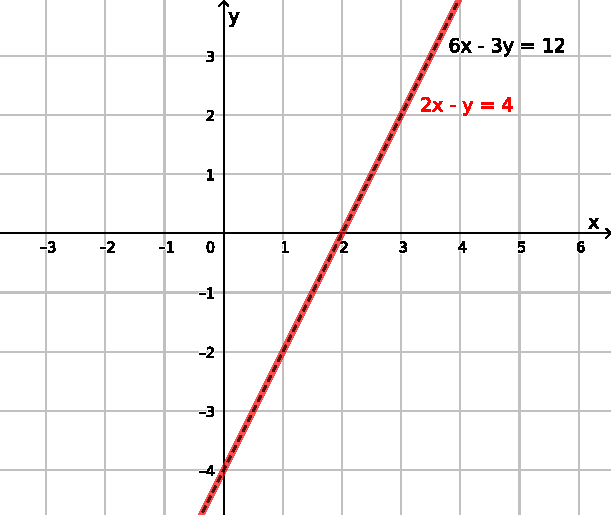
\includegraphics[width=7cm]{../../Topicos/Figuras/Sistema_(SPI).pdf}}
    \caption{Sistema possível Indeterminado}
  \end{figure}
 \end{exem}

 \item \textbf{2º caso: Retas Paralelas}

 Se existe $\alpha \in \R$ tal que $a_1= \alpha a_2$, $b_1= \alpha b_2$ e $c_1 \neq \alpha c_2$, então as equações do sistema tem coeficientes múltiplos, mas as constantes $c_1$ e $c_2$ não são múltiplas, consequentemente seus gráficos são \textbf{retas paralelas}, que nunca se intersectam, logo o sistema não possui soluções, sendo portanto um {\color{red} Sistema impossível (SI)}.

\begin{exem}
 Situação esta presente por exemplo no seguinte sistema de equações lineares:
 \[\begin{cases}
    2x - y= -2 \\
    2x - y= 4
   \end{cases}
\]
que é representado geometricamente na figura abaixo:

 \begin{figure}[H]
 \centering
    \fbox{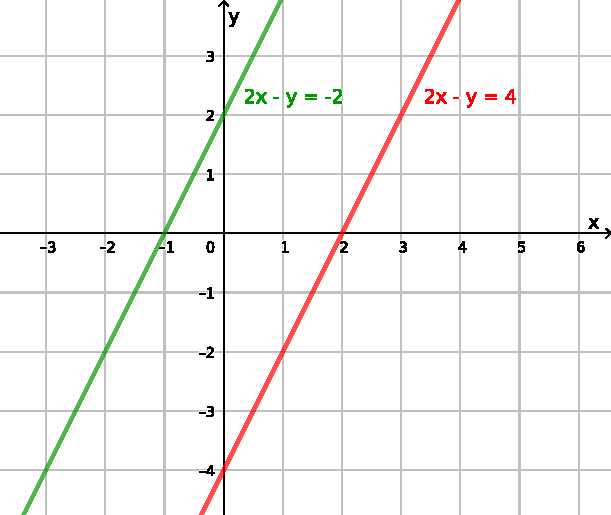
\includegraphics[width=7cm]{../../Topicos/Figuras/Sistema_(SI).pdf}}
    \caption{Sistema impossível}
  \end{figure}
 \end{exem}

 \item \textbf{3º caso: Retas Concorrentes}

 Caso nenhuma das duas situações acima ocorra, temos que as equações do sistema possuem como gráficos \textbf{retas concorrentes} e que concorrem em um único ponto, o qual é a solução do nosso sistema, este é portanto um {\color{red} sistema possível determinado (SPD)}.

 \begin{exem}
 Um exemplo desta situação é o sistema;
 \[\begin{cases}
    2x - y= 4 \\
    x + 2y= -3
   \end{cases}
\]
que foi utilizado anteriormente como exemplo das duas possíveis formas de resolver um sistema linear. Onde vimos que sua solução é dada pelo par ordenado $(1, -2)$. Abaixo temos representação geométrica deste sistema, na qual é possível observar que a interseção das duas retas se dá exatamente no ponto $(1, -2)$:

  \begin{figure}[H]
 \centering
    \fbox{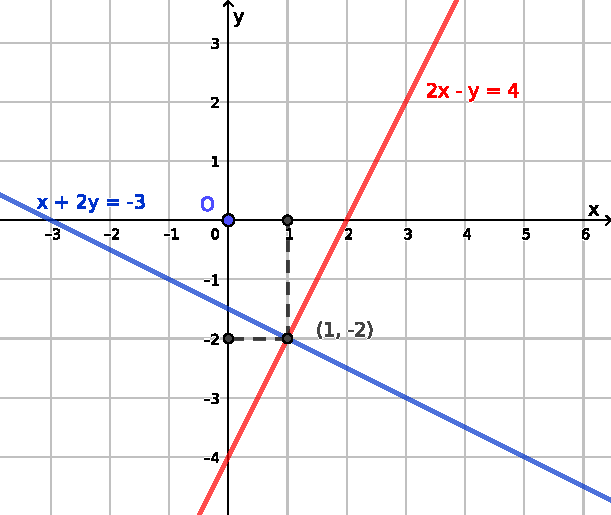
\includegraphics[width=7cm]{../../Topicos/Figuras/Sistema_(SPD).pdf}}
    \caption{Sistema possível determinado}
  \end{figure}
 \end{exem}

 \end{itemize}

 Resumindo os sistemas lineares $2 \times 2$ podem ser classificados de acordo com suas soluções da seguinte forma:

 \begin{figure}[H]
  \centering
  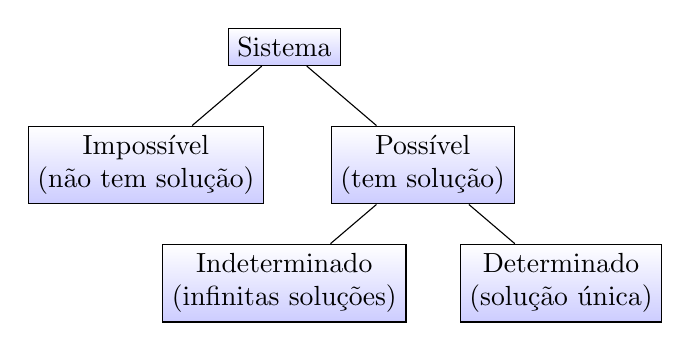
\begin{tikzpicture}[grow'=down,sibling distance=8em,
  level 1/.style={sibling distance=10em},
  level 2/.style={sibling distance=10em},
  every node/.style = {shape=rectangle, draw, align=center, top color=white, bottom color=blue!20}]]

  \node {Sistema}
    child { node {Possível \\ (tem solução)}
             child { node {Determinado \\ (solução única)} }
             child { node {Indeterminado \\  (infinitas soluções)} } }
    child { node {Impossível \\ (não tem solução)}};
 \end{tikzpicture}
 \end{figure}




\section{Sistema de três equações lineares}

\vskip0.3cm
 \colorbox{azul}{
 \begin{minipage}{0.9\linewidth}
  Em particular uma equação em três variáveis $x$, $y$ e $z$ é da forma $ax + by + cz= d$ onde $a, b, c$ e $d$ são constantes reais e $a$, $b$ e $c$ não são simultaneamente nulos. Assim ao consideramos três destas equações
  \[S= \begin{cases}
      a_1x + b_1y + c_1z= d_1 \\
      a_2x + b_2y + c_2z= d_2 \\
      a_3x + b_3y + c_3z= d_3
     \end{cases}\]
 temos um sistema linear de três equações lineares e três incógnitas. Uma tripla de valores $x$, $y$ e $z$, frequentemente representada pela tripla ordenada $(x, y, z)$, que satisfaz as três equações, quando existe, é chamada de solução do sistema.
 \end{minipage}}
 \vskip0.3cm




\begin{exem}
 Considere o sistema $S_1$ dado por:
 \[S_1= \begin{cases}
      -x + y + z= -1 \\
      x + y + z= -1 \\
      x - y + z= -1,
     \end{cases}\]
 note que a tripla ordenada $(0, 0, -1)$ é solução deste sistema já que:
 \[S_1= \begin{cases}
      - 0 + 0 -1 = -1 \\
      0 + 0 -1 = -1\\
      0 - 0 -1 = -1
     \end{cases} .\]

Já a tripla ordenada $(-1, 0, 0)$ não é solução do sistema $S_1$ pois:
\[S_1= \begin{cases}
      -(-1) + 0 + 0= 1 \neq -1 \\
      -1 + 0 + 0 = -1 \\
      -1 -0 + 0 = -1
     \end{cases} .\]
\end{exem}

Os métodos da adição/subtração e método da substituição apresentados para resolução de sistemas lineares $2 \times 2$ podem ser utilizados também para resolver sistemas lineares $3 \times 3$. O seguinte exemplo ilustra a resolução de um sistema linear $3 \times 3$ pelo método da adição:

\begin{exem}
 \[S_1= \begin{cases}
         x + y + z= 3 \ \ \ (I)\\
         -x - y + 2z= 0 \ \ \ (II)\\
         -x + 3y + z= 3 \ \ \ (III)
        \end{cases} \]

 Primeiramente vamos fazer (equação I + equação III) e depois (equação II - equação III), com isso eliminamos a variável $x$ e ficamos com duas equações das variáveis $y$ e $z$.

 equação I + equação III:
 \[\begin{tabular}{cccccccc}
   & x & +  & y & + & z & =  & 3  \\
 + & -x & + & 3y & + & z & = & 3 \\\hline
   & 0 & + & 4y & + & 2z & = & 6 \ \ \ (IV)\\
\end{tabular}\]

equação II - equação III:
\[\begin{tabular}{cccccccc}
   & -x & - & y & + & 2z & = & 0 \\
 - & -x & + & 3y & + & z & = & 3 \\\hline
   & 0 & - & 4y & + & z & = & -3 \ \ \ (V)\\
\end{tabular}\]

Obtemos assim o seguinte sistema linear:
\[S'= \begin{cases}
       4y + 2z = 6 \\
       -4y + z= -3
      \end{cases}\]

 Façamos então a soma destas equações para eliminar $y$, da seguinte forma:
 \[\begin{tabular}{cccccccc}
   & 4y & + & 2z & = & 6 \\
 + & -4y & + & z & = & -3 \\\hline
   & 0 & + & 3z & = & 3 \\
\end{tabular}\]
Com isso chegamos em:
\[\Rightarrow 3z= 3 \Rightarrow z= \frac{3}{3} \Rightarrow z= 1 \]
Voltando o valor de $z$ na equação $(IV)$ ou $(V)$ obtemos o valor de $y$, façamos então usando a equação $(V)$:
\[(V) -4y + z = -3 \Rightarrow -4y + 1 = -3 \Rightarrow -4y = -3 - 1 \Rightarrow -4y = -4 \Rightarrow y = 1.\]
Agora retornamos com os valores de $y$ e $z$ na equação $(I)$ para determinar o valor de $x$;
\[(I) x + y + z= 3 \Rightarrow x + 1 + 1 = 3 \Rightarrow x = 3 - 2 \Rightarrow x = 1.\]
Portanto a terna ordenada $(x, y, z)= (1, 1, 1)$ é solução deste sistema linear.
\fim

\end{exem}

Vale observar que assim como no caso dos sistemas $2 \times 2$, os sistemas $3 \times 3$ também possuem uma interpretação geométrica, já que uma equação da forma $ax + by + cz = d$, para $a, b, c, d \in \R$, tais que $a^2 + b^2 + c^2 \neq 0$, ou seja, tais que $a, b, c$ não são todos nulos, representa um plano em $\R^3$. Logo, dado um sistema linear
\[S= \begin{cases}
      a_1x + b_1y + c_1z= d_1 \\
      a_2x + b_2y + c_2z= d_2 \\
      a_3x + b_3y + c_3z= d_3
     \end{cases}\]
temos que cada uma das equações, nessa ordem, definem os planos $\pi_1$, $\pi_2$ e $\pi_3$, respectivamente. Portanto a resolução deste tipo de sistema linear também possui uma interpretação geométrica que depende da posição relativa destes planos em $\R^3$.

Podemos classificar os sistemas $3 \times 3$ de acordo com suas soluções da seguinte forma:

 \begin{figure}[H]
  \centering
  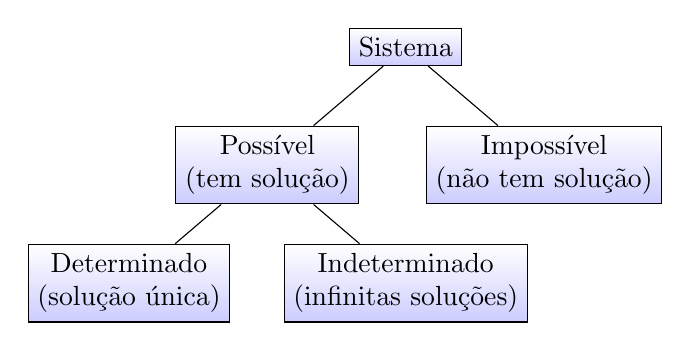
\begin{tikzpicture}[grow'=down,sibling distance=8em,
  level 1/.style={sibling distance=10em},
  level 2/.style={sibling distance=10em},
  every node/.style = {shape=rectangle, draw, align=center, top color=white, bottom color=blue!20}]]

  \node {Sistema}
    child { node {Impossível \\ (não tem solução)}}
    child { node {Possível \\ (tem solução)}
             child { node {Indeterminado \\  (infinitas soluções)} }
             child {  node {Determinado \\ (solução única)} } };
 \end{tikzpicture}
 \end{figure}

 e estas soluções podem ser interpretadas geometricamente, façamos as interpretações geométricas em cada um dos três casos:
 \begin{itemize}
  \item \textbf{Sistema possível determinado (SPD)}: existe uma única solução para o sistema;
  \begin{itemize}
    \item  Os três planos tem um único ponto em comum $\pi_1 \cap \pi_2 \cap \pi_3= \{P\}$.
  \end{itemize}

  \item \textbf{Sistema possível indeterminado (SPI)}: existem infinitas soluções para o sistema;
  \begin{itemize}
    \item Os três planos coincidem: assim, todos os pontos $P(x, y, z)$ de $\pi_1$ são soluções do sistema.

    \item Dois planos coincidem e o terceiro os intersecta segundo uma reta: todos os pontos $P(x, y, z)$ da reta são solução para o sistema.

    \item Os três planos são distintos e tem uma reta em comum $\pi_1 \cap \pi_2 \cap \pi_3= \{r\}$: logo, todos os pontos $P(x, y, z)$ da reta $r$ são soluções do sistema.
  \end{itemize}

  \item \textbf{Sistema impossível (SI)}: o sistema não possui solução;
  \begin{itemize}
  \item Dois planos coincidem e o terceiro é paralelo: não há nenhum ponto na interseção dos três planos.

  \item Os planos são paralelos dois a dois: não há nenhum ponto na interseção dos três planos.

  \item Dois planos são paralelos e o outro os intersecta segundo retas paralelas $r$ e $s$: podemos ter por exemplo, $\pi_1$ paralelo à $\pi_2$, portanto $\pi_1 \cap \pi_2 = \emptyset$,  logo, $\pi_1 \cap \pi_2 \cap \pi_3 = \emptyset$, ou seja, o sistema não tem solução.

  \item Os três planos se intersectam, dois a dois, segundo retas paralelas umas às outras.
  \end{itemize}

 \end{itemize}

\newpage
